\section{Related Work}\label{Section_related_work}

\subsection{Vision-Language-Action (VLA) Models} \label{Subsection_VLA}
Recently, leveraging pre-trained Vision-Language Models (VLMs) \citep{Prismatic-2024, PaliGemma-2024, LLaVA-2023, Eagle-2-2025} to control robots for performing various daily tasks has substantially accelerated research in embodied intelligence. This has emerged as a prominent research focus \citep{pi0-2025, pi0.5-2025, SmolVLA-2025, GR00T-N1-2025, RDT-2025, Being-H0-2025, GR3-2025, G0-2025, QUAR-2024, CLOVER-2024, LongVLA-2025, QUARTOnline-2025}. These models are referred to as the VLA models.

Typically, VLA models require large-scale embodied datasets, such as Open X-Embodiment \citep{OpenX-2024}, for pre-training \citep{RDT-2025, GR3-2025}. This process integrates VLMs with a dedicated Policy network \citep{Hume-2025, RoboFlamingo-2024}, allowing the system to decode or generate action sequences for diverse tasks in an end-to-end manner. Moreover, dual-system VLA architectures \citep{LCB-2024, RoboDual-2024, OpenHelix-2025} have recently garnered attention. These methods typically introduce an intermediate latent token to connect the VLMs and the Policy, using an asynchronous mechanism to enhance coordination between the two systems \citep{HiRT-2024}. This design mitigates latency issues during action generation.

Consequently, how to effectively and efficiently bridge the gap from the vision-language perception space to the action space has become a key challenge in the design of VLA models.


\subsection{Bridging from Perception to Action Space} \label{sec22} 
Earlier studies \citep{OpenVLA-2024, RT-2-2023, RT-1-2023} attempted to directly align perception and action spaces by discretizing actions into tokens. However, this discretization inevitably introduces inherent loss. Recent studies have shifted their focus toward continuous action spaces \citep{RoboVLMs-2024, GR00T-N1-2025, pi0-2025, SmolVLA-2025, OpenVLA-OFT-2025}. Based on the types of perceptual features utilized to bridge to the action space, they can be categorized:

\paragraph{1) Raw Features from VLMs.} Raw features (refer to vision and language representations) are extracted directly from the VLM. Early methods extract representations from the final-layer VLM, operating under the assumption that it encodes the most task-relevant semantic information \citep{RoboVLMs-2024, HiRT-2024}. More recent methods leverage the intermediate-layer features within the VLM \citep{pi0-2025}. They believe that such representations may retain richer multimodal information, thereby benefiting Policy in tasks that demand fine-grained perception or complex reasoning. For example, some studies use features from a middle layer \citep{GR00T-N1-2025}, the first-half layers \citep{SmolVLA-2025}, or all intermediate-layer features \citep{pi0-2025}.

\paragraph{2) Additional Query as Interface.} Furthermore, recent studies \citep{OpenVLA-OFT-2025, OpenHelix-2025} have introduced a novel interface that employs additional queries as bridges between VLMs and Policy, rather than transmitting Raw features. The query is learnable and can incorporate multimodal information, showing superior performance. The existing bridge paradigms are shown in Figure \ref{Figure_mapping}.


\begin{figure}[!htbp]
	\centering
	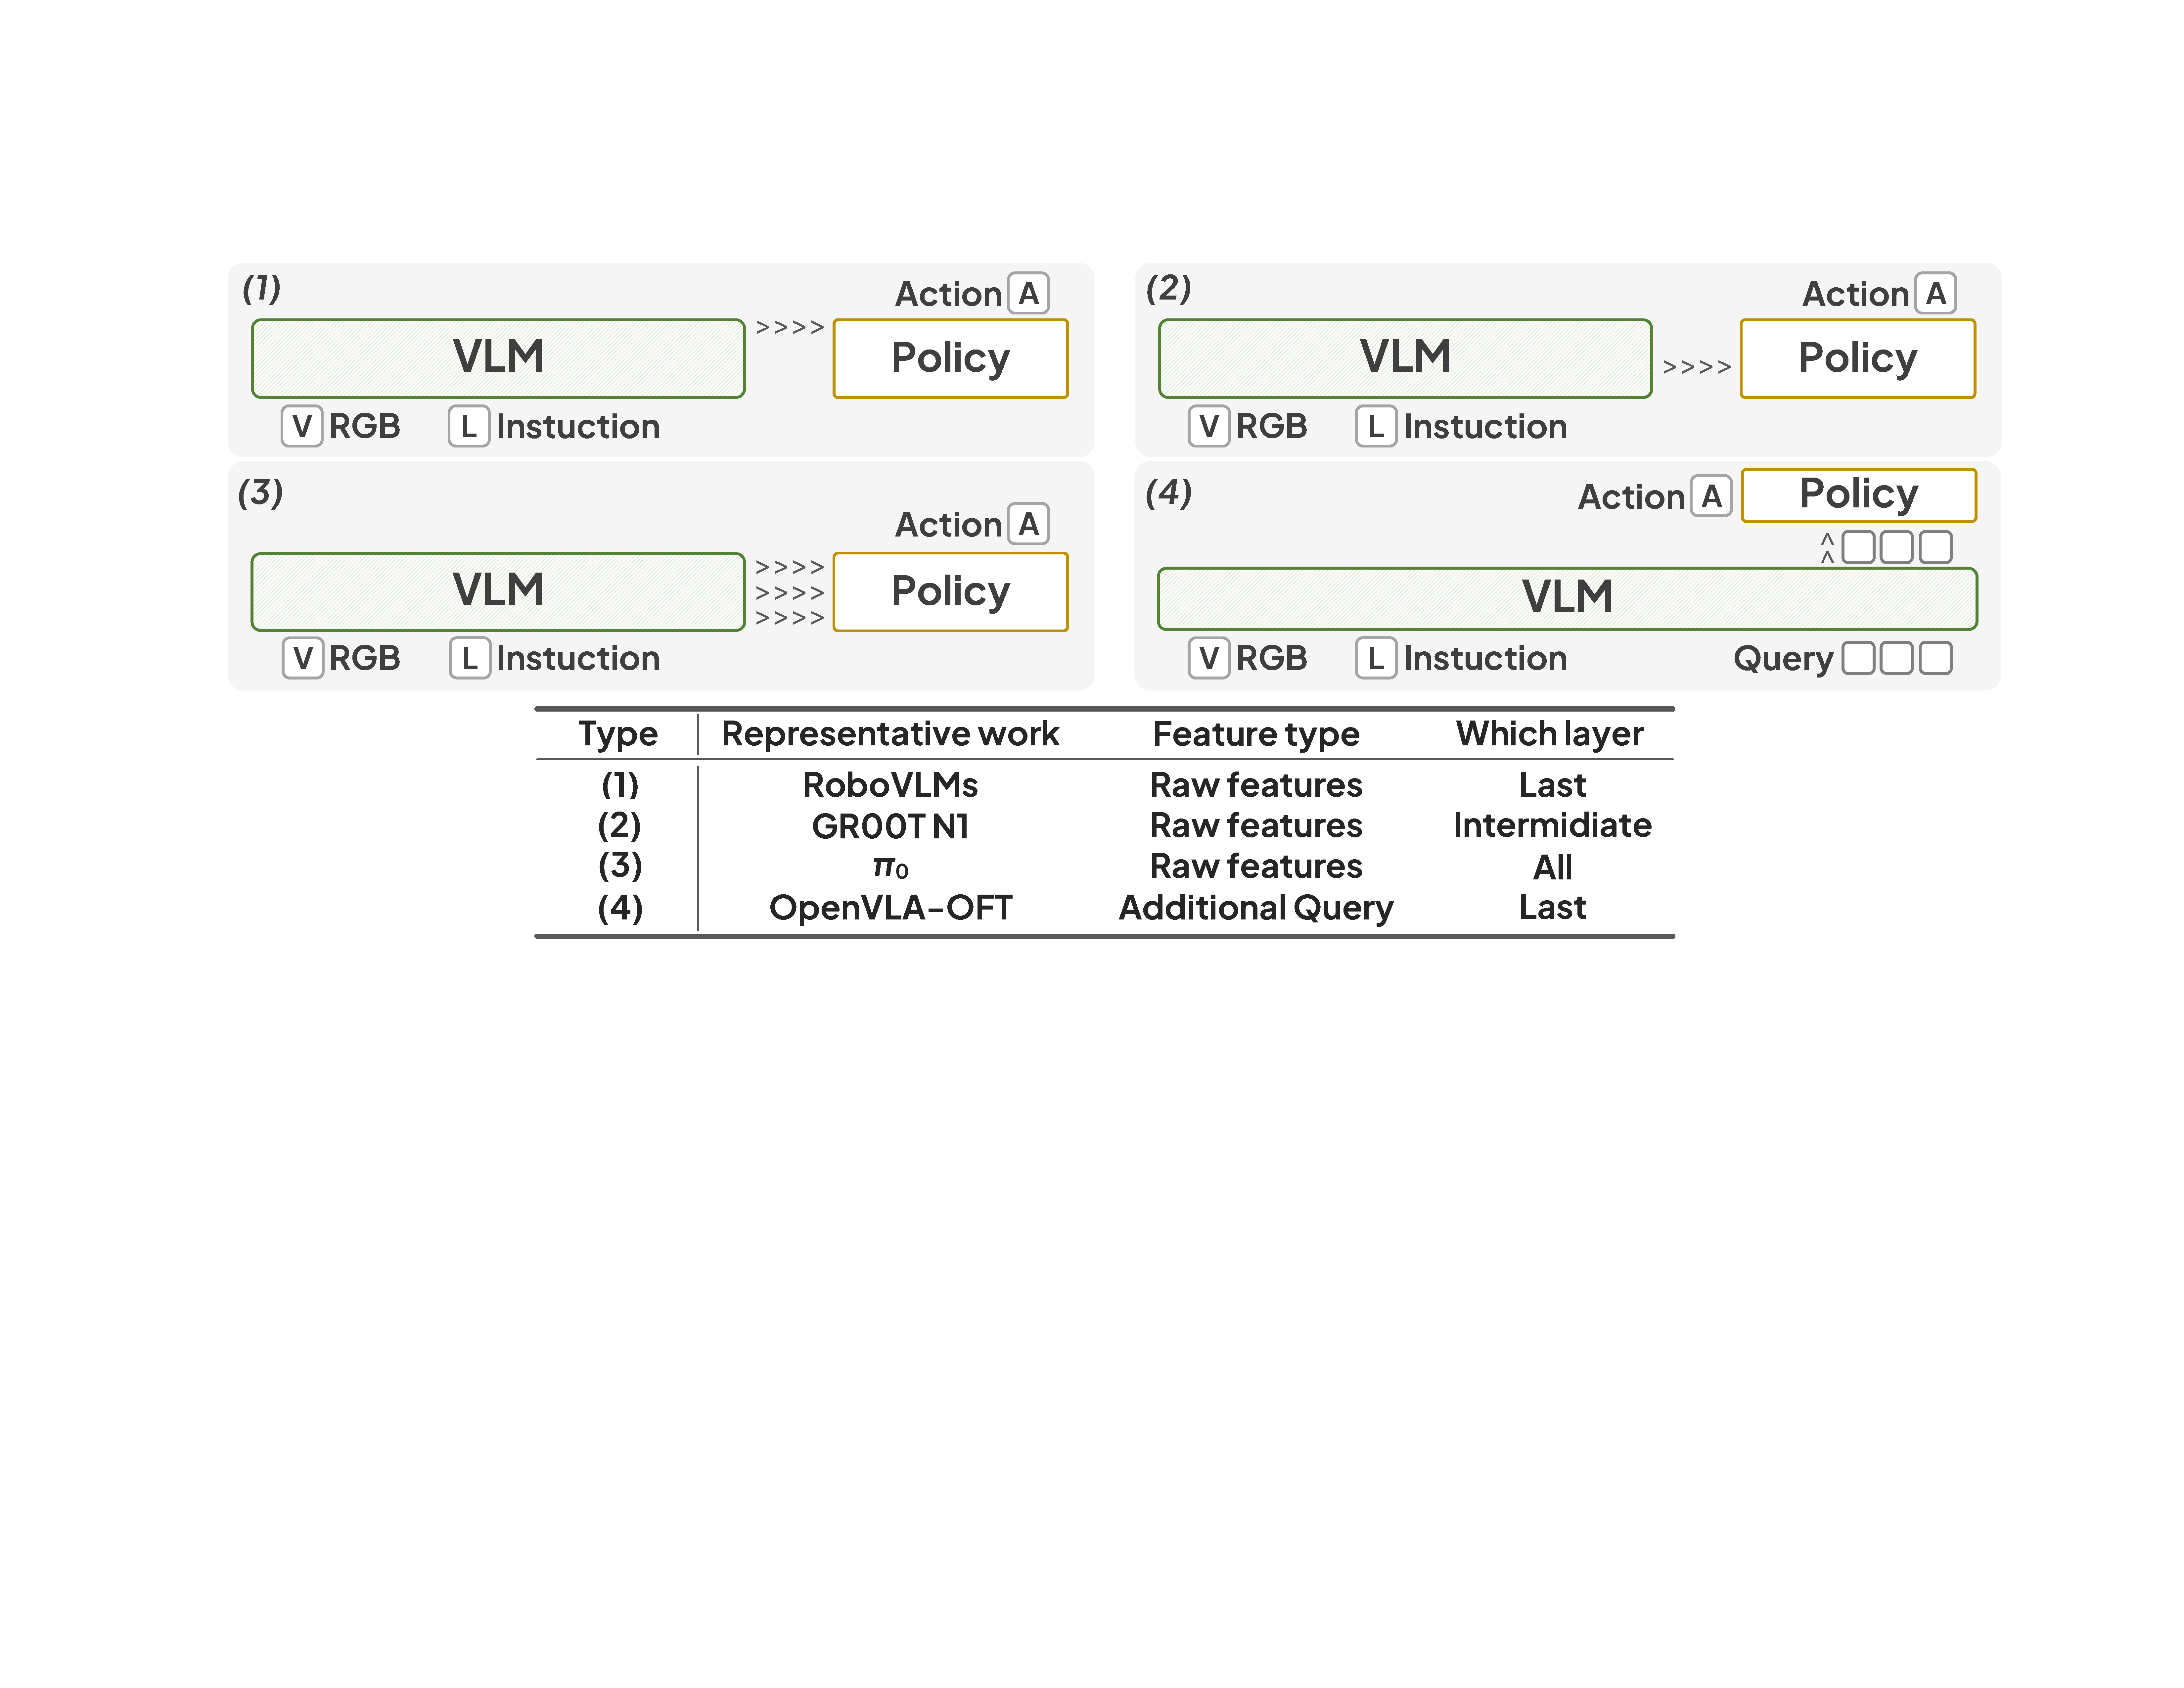
\includegraphics[width=0.95\textwidth]{Figures/Mapping1.pdf}	
	\caption{Existing representative bridge paradigms from VL to A.}\label{Figure_mapping}
\end{figure}